\documentclass[a4paper,12pt]{article} 

\usepackage[top = 2.5cm, bottom = 2.5cm, left = 2.5cm, right = 2.5cm]{geometry} 

\usepackage[T1]{fontenc}
\usepackage[utf8]{inputenc}
\usepackage{amsmath}
\usepackage{multirow}
\usepackage{booktabs} 
\usepackage{tikz}
\usepackage{graphicx} 
\usepackage{amssymb} 
\usepackage{pdfpages}

\usepackage{setspace}
\setlength{\parindent}{0in}

\usepackage{float}

\usepackage{fancyhdr}
\usepackage{enumerate}


\pagestyle{fancy} 
\fancyhf{}
\lhead{\footnotesize PR \& ML: Blatt 1}
\rhead{\footnotesize F. Freter, E. Kirchberger, S. Symhoven \& J. Wustl} %<---- Fill in your lastnames.

\cfoot{\footnotesize \thepage} 

\begin{document}

\thispagestyle{empty} 

\begin{tabular}{p{15.5cm}} 
{\large \bf Pattern Recognition und Machine Learning} \\
Hochschule München \\ Sommersemester 2023  \\ Prof. Dr.-Ing. Claudius Schnörr \\
\hline 
\\
\end{tabular} 

\vspace*{0.3cm} 

\begin{center} 
	{\Large \bf Blatt 1} 
	\vspace{2mm}
	

	{\bf F. Freter, E. Kirchberger, S. Symhoven \& J. Wustl} 
		
\end{center}  

\vspace{0.4cm}

\section*{Aufgabe 2a: Statistik}

\begin{enumerate}

\item {Dichte, Erwartungswert, Varianz und Kovarianz

	\begin{enumerate}[a)]

		\item Die Dichte der gleichverteilten 1D-Zufallsvariable $x$ im Intervall $[a,b] \subset \mathbb{R}$ ist definiert als:
			
		\begin{equation*}
			p(x) = \begin{cases}
       				\frac{1}{b-a} & \text{für } a \leq x \leq b \\
         			0 & \text{sonst}
       			\end{cases} 
		\end{equation*}
		
		und kann wie folgt skizziert werden:
		
		\begin{tikzpicture}[scale=1.5]
			\draw[->] (-0.5,0) -- (3,0) node[right] {$x$};
			\draw[->] (0,-0.5) -- (0,1.5) node[above] {$p(x)$};
			\draw[thick] (1,0) -- (1,1) -- (2,1) -- (2,0);
			\draw[dashed] (1,0) node[below] {$a$} -- (1,1);
			\draw[dashed] (2,0) node[below] {$b$} -- (2,1);
			\node at (3,0.5) {$p(x) = \frac{1}{b-a}$};
		\end{tikzpicture}
		
		Die Dichte auf dem Intervall $[a,b]$ hat den Wert $\frac{1}{b-a}$.

		\item Erwartungswert:
		
		\begin{align*}
			E[X] &= \int_{-\infty}^{\infty} x \, p(x) \, dx \\
			&= \int_a^b x \cdot \frac{1}{b-a} \, dx \\
			&= \frac{1}{b-a} \cdot \left[ \frac{x^2}{2} \right]_a^b \\
			&= \frac{b^2 - a^2}{2(b-a)} \\
			&= \frac{a+b}{2}
		\end{align*}

		\item Varianz 
		
		\begin{align*}
			Var(X) &= E[(x - \mu_x)^2] \\
			&= \int_a^b (x-\mu_x)^2 \, p(x) \, dx \\
			&= \int_a^b (x - \frac{a+b}{2})^2 \cdot \frac{1}{b-a} \, dx \\
			&= \left[ \frac{1}{3} (x - \frac{a+b}{2})^3 \cdot \frac{1}{b-a} \right]_a^b \\
			&= \frac{1}{3(b-a)} \left( (b - \frac{a+b}{2})^3 - (a - \frac{a+b}{2})^3 \right) \\
			&= \frac{1}{3(b-a)} \left( (\frac{b-a}{2})^3 + (\frac{b-a}{2})^3 \right) \\
			&= \frac{1}{3(b-a)} 2(\frac{b-a}{2})^3 \\
			&= \frac{2(\frac{b-a}{2})^3}{3(b-a)} \\
			&= \frac{2}{3}\frac{(\frac{b-a}{2})^3}{(b-a)} \\
			&= \frac{1}{12} \cdot (b-a)^2
		\end{align*}

	\end{enumerate}

}

\item {Sample Mean und Kovarianzmatrix

	\begin{enumerate}[a)]

		\item 
		
		\begin{align*}
			\mu_X &= \frac{1}{n} \sum_{i} X_i \\
			&= \frac{1}{4} \sum_{i=1}^{4} X_i \\
			&= \frac{1}{4} * \left[ \left(\begin{array}{c} 1 \\ 2 \end{array}\right) + \left(\begin{array}{c} -1 \\ -1 \end{array}\right) + \left(\begin{array}{c} -5 \\ 1 \end{array}\right) + \left(\begin{array}{c} 1 \\ 2 \end{array}\right) \right] \\
			&= \frac{1}{4} \left(\begin{array}{c} -4 \\ 4 \end{array}\right) \\
			&= \left(\begin{array}{c} -1 \\ 1 \end{array}\right)
		\end{align*}
		
		\item
		
		\begin{align*}
    			\sum_{\mathbf{xx}} &= \frac{1}{n}\sum_{i=1}^{n}(\mathbf{x}_i - \mu_{\mathbf{x}})(\mathbf{x}_i - \mu_{\mathbf{x}})^T \\
     				&= \frac{1}{4}\left[ \begin{pmatrix} 2 \\ 1 \end{pmatrix}\begin{pmatrix} 2 & 1 \end{pmatrix} + \begin{pmatrix} 0 \\ 2 \end{pmatrix}\begin{pmatrix} 0 & 2 \end{pmatrix} + \begin{pmatrix} -4 \\ 0 \end{pmatrix}\begin{pmatrix} -4 & 0 \end{pmatrix} + \begin{pmatrix} 2 \\ 1 \end{pmatrix}\begin{pmatrix} 2 & 1 \end{pmatrix}\right] \\
     				&= \frac{1}{4}\left[ \begin{pmatrix} 4 & 2 \\ 2 & 1 \end{pmatrix} + \begin{pmatrix} 0 & 0 \\ 0 & 4 \end{pmatrix} + \begin{pmatrix} 16 & 0 \\ 0 & 0 \end{pmatrix} + \begin{pmatrix} 4 & 2 \\ 2 & 1 \end{pmatrix}\right] \\
     				&= \frac{1}{4} \begin{pmatrix} 24 & 4 \\ 4 & 6 \end{pmatrix} \\
     				&= \begin{pmatrix} 6 & 1 \\ 1 & 1.5 \end{pmatrix} \\
		\end{align*}
		


	\end{enumerate}

}

\item {Multivariate Normalverteilung

	\begin{enumerate}[a)]

		\item Die beiden Verteilungen der Zufallsvariablen $\mathbf{u}$ und $\mathbf{v}$ liegen wie folgt im x/y-Koordinatensystem.
		Die Verteilung der Zufallsvariable $\mathbf{u}$ entspricht der horizontalen Ellipse links. Diese hat den Mittelpunkt im Ursprung, eine Varianz von 4 in x-Richtung und eine Varianz von 2 in y-Richtung.
		Die Verteilung der Zufallsvariable $\mathbf{v}$ entspricht der vertikalen Ellipse rechts. Diese hat den Mittelpunkt um 4 in x-Richtung verschoben, eine Varianz von 2 in x-Richtung und eine Varianz von 4 in y-Richtung:
		
		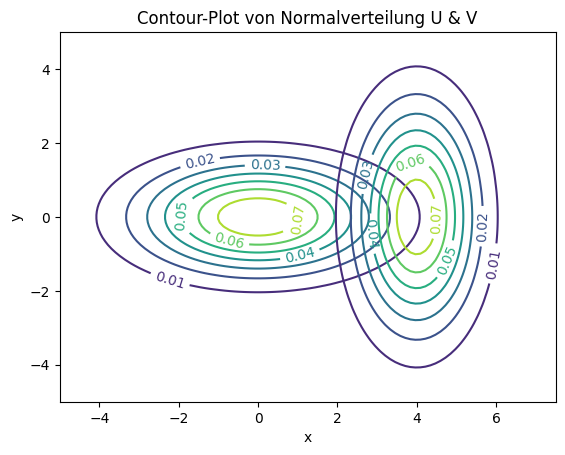
\includegraphics{3a.png}

		\item 
		
		Die Trennfunktion muss eine Funktion sein, die die Grenze zwischen den beiden Verteilungen darstellt. 

		Bei einer Bayes-Entscheidungsregel lautet die Trennfunktion:

		\begin{equation}
			T(x) = \log\left(\frac{p(x|C_1)}{p(x|C_2)}\right) + \log\left(\frac{p(C_2)}{p(C_1)}\right)
		\end{equation}

		mit $p(x|C_i)$ als der Wahrscheinlichkeit, dass $x$ in der Klasse $C_i$ liegt, und $p(C_i)$ als der A-priori-Wahrscheinlichkeit der Klasse $C_i$.

		Da in diesem Fall die A-priori-Wahrscheinlichkeiten der beiden Verteilungen gleich sind, vereinfacht sich die Gleichung zu:

		\begin{equation}
			T(x) = \log\left(\frac{p(x|U)}{p(x|V)}\right)
		\end{equation}

		Die Trennfunktion sieht dann wie folgt aus:

		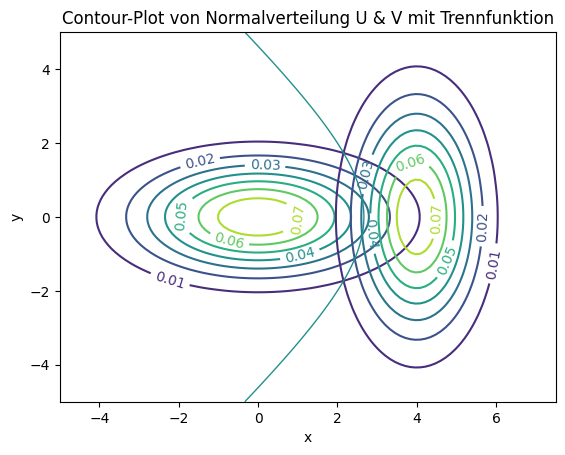
\includegraphics{3b.png}

	\end{enumerate}

}

\item {Entropie einer diskreten Verteilung

	\begin{enumerate}[a)]

		\item 
		
		\begin{align*}
			E[ln(x) \mid x = 1] = ln(1) = 0
		\end{align*}

		\item 
		
		\begin{align*}
			E[ln(x) \mid x = 2] = ln(2) \approx 0.6931
		\end{align*}
		
		\item
		
		\begin{align*}
			H(X) &= - \sum P(x) \cdot \ln(P(x)) \\
				 &= - [P(1) \cdot \ln(P(1)) + P(2) \cdot \ln(P(2))] \\
     			 &= - [0,2 \cdot \ln(0,2) + 0,8 \cdot \ln(0,8)] \\
     			 &\approx 0,5004
		\end{align*}
		
		\item
		
		\begin{align*}
			H(X) &= - \sum P(x) \cdot \ln(P(x)) \\
				 &= - [P(1) \cdot \ln(P(1)) + P(2) \cdot \ln(P(2))] \\
     			 &= - [0,1 \cdot \ln(0,1) + 0,9 \cdot \ln(0,9)] \\
     			 &\approx 0,4689
		\end{align*}
		
		Die Entropie ist etwas niedriger als zuvor, was darauf hindeutet, dass die Verteilung jetzt etwas vorhersehbarer ist. 
		Das macht Sinn, da die Wahrscheinlichkeit für Ereignis $P_2$ gestiegen und für $P_1$ gefallen ist. Dass $P_2$ eintritt, ist
		nun also sicherer als vorher und die Entropie somit geringer, da das Ergebnis vorhersehbarer wird.

	\end{enumerate}

}

\end{enumerate}

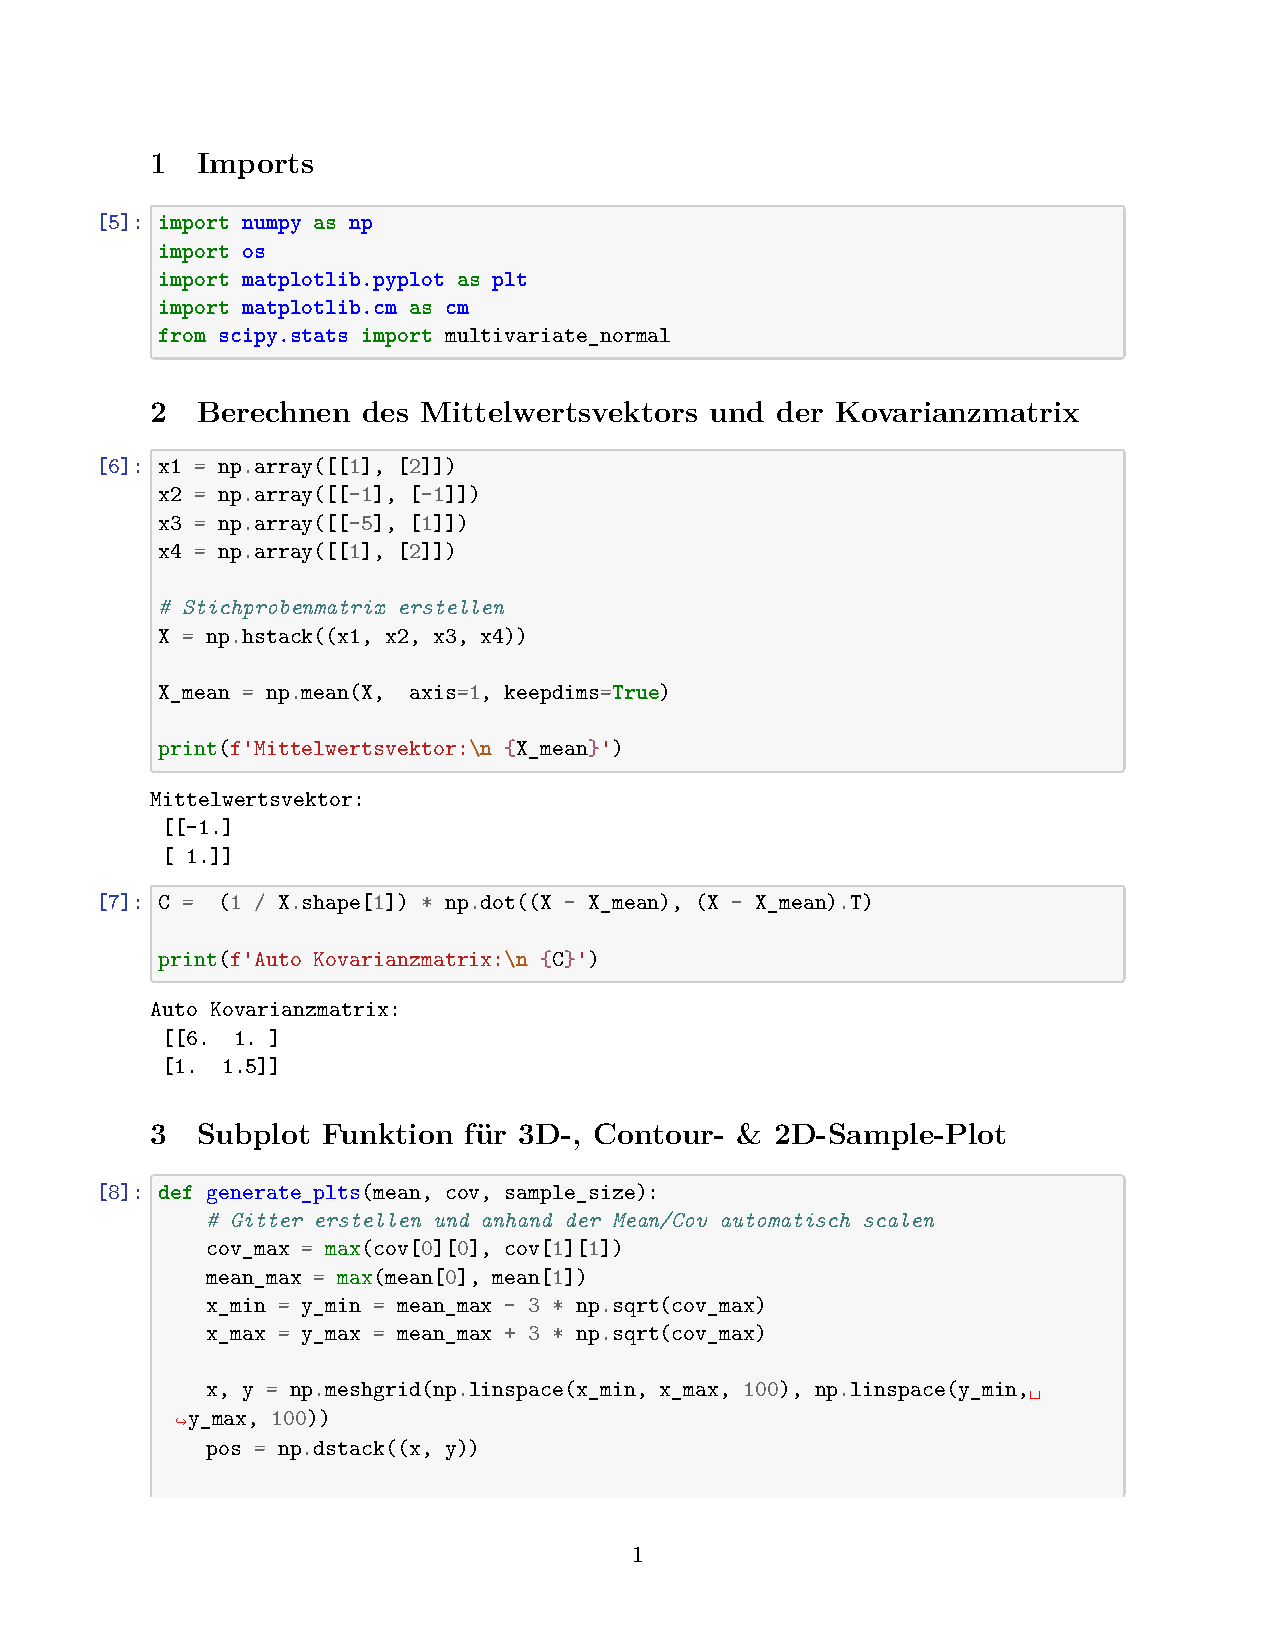
\includepdf[pages=1,pagecommand=\section*{Aufgabe 2b: Statistik}]{aufgabe-2.pdf}
\includepdf[pages={2-}]{aufgabe-2.pdf}

\end{document}
